\chapter{AsthmaBuddy}
\label{chp:our-solution}

\section{Background}
As mentioned in Chapter \ref{chp:background}; in 2012, we did a similar project using Karotz\fnurl{Karotz}{www.karotz.com} as the platform for the tangible user interface\cite{CustomerDriven}.
This project left us with mixed feelings towards Karotz as a platform. The thought behind Karotz is great. It is an open source robot which allows people to build applications and launch it to the Karotz store. However, in our subjective opinion, it is not ideal to work with. Firstly, the Karotz starters kit costs ~200 USD. Thus it is a pretty large investment for a family wanting to use our application. Secondly, the API is only documented in French, which limits the number of developers who are willing to develop applications for the Karotz. Thirdly, the Karotz is pretty cumbersome to configure for a person with little knowledge of computer configurations, e.g. the Karotz requires SSH access (Secure SHell access) for initial configurations. Fourthly, we did not want our product to be constrained by the limitations of the Karotz.

We researched other alternatives in order to create a tangible user interface from scratch and we looked into was Arduino and Raspberry Pi. Arduino is an open source electronics prototyping platform\cite{arduino}, which allows for many different combinations of configurations. Arduino shields comes in many shapes and sizes and is built for modularity and extendability. A wide range of components are available if one wishes to add technical functionality to an Arduino system, such as Bluetooth, WiFi or small motors. 
While Arduino allows complex hardware configurations, Raspberry Pi makes larger abstractions, which seemed like the better choice for us as developers. Arduino programs are normally written in C\cite{strahl2000language}, which we had little to no prior experience with. Additionally, Arduinos generally have low-powered CPUs, in order to keep them cheap. These low-powered CPUs tend to have problems with decoding MP3-files, which would lay heavy constraints to our system (without using sounds or a display, it is hard to communicate with children). Due to these facts, we choose to develop the system on a Raspberry Pi.

Our tangible user interface was planned to have similar functionality to what KAPP had, with some modifications. 
 
\section{Technology}
\label{sec:technology}

\subsection{Raspberry Pi - Specifications Overview}
The \rpi{} was initially intended to teach british school children about computer programming\cite{rasperrypi-about}. Since its release, it took an unexpected turn when a large number of computer enthusiasts bought the product to do their own mini projects for a cheap price. 

The specification of a \rpi{} (Model B) is included in Table \ref{tab:pi-specs}. Figure \ref{fig:pi-arch-overview} shows an overview of the \rpi{}.        

\begin{table}[H]
\centering
\begin{tabular}{|p{6.0cm} | p{6.0cm} |}
\hline 
\textbf{Property} & \textbf{Specification} \\
\hline
CPU & 700 MHz ARM1176JZF-S core \\
\hline
Memory & 512 MB \\
\hline
USB 2.0 ports & 2 \\
\hline
Video Output & HDMI \\
\hline
Audio Output & 3.5 mm jack, in addition to ability to play sound through HDMI \\
\hline
Low-level Peripherals & 8 x GPIO (General Purpose Input/Output) \\
\hline
Power Source & 5 volt MicroUSB \\
\hline
Storage & SD card (available with preinstalled OS) \\
\hline
Network & 10/100 Mbps Ethernet  \\
\hline
\end{tabular}
\caption{Raspberry Pi specifications}
\label{tab:pi-specs}
\end{table}

\begin{figure}[H] 
	\begin{minipage}[t]{0.4\linewidth}
	\centering
		\fbox{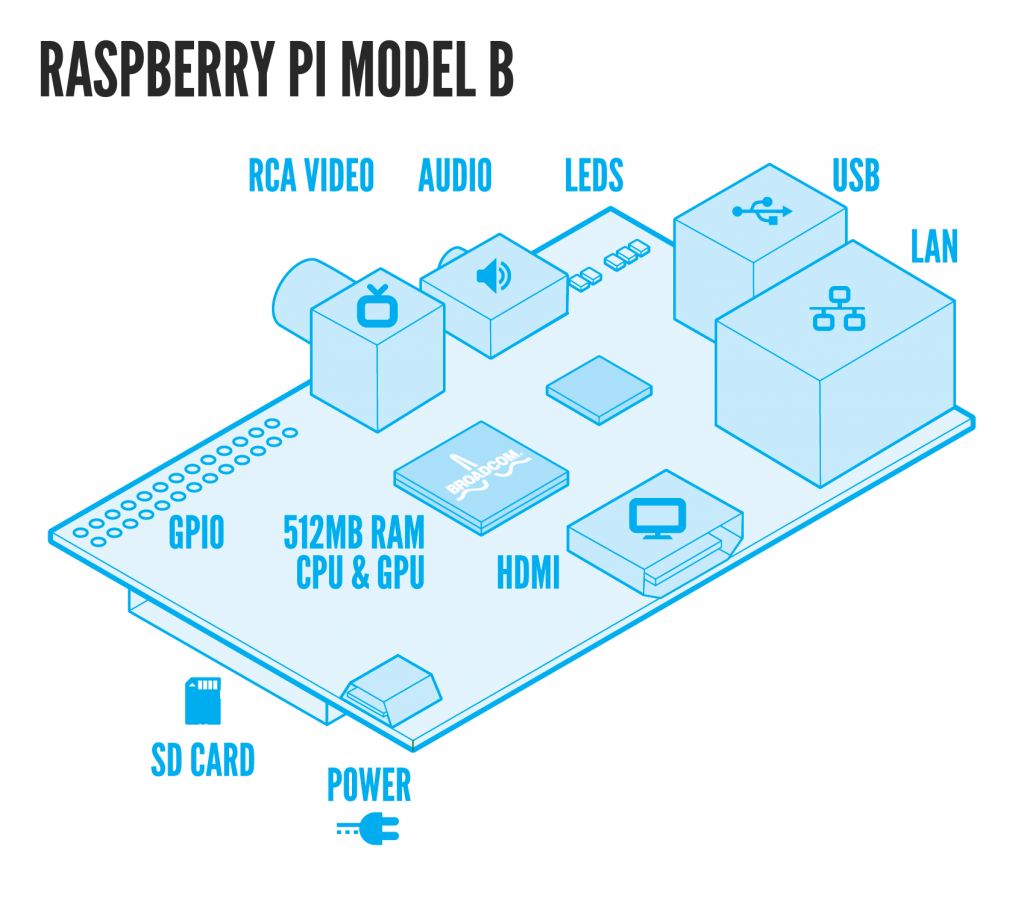
\includegraphics[width=0.3\paperwidth]{Pictures/rpi-arch-overview.png}}
	\caption[Raspberry Pi Model B Architecture]{Raspberry Pi Model B architecture.}
	\caption*{Image source: \url{http://raspberrypi.org/faqs}}
	\label{fig:pi-arch-overview}
	\end{minipage}
	\hspace{2.0cm}
	\begin{minipage}[t]{0.4\linewidth}
		\centering
			\fbox{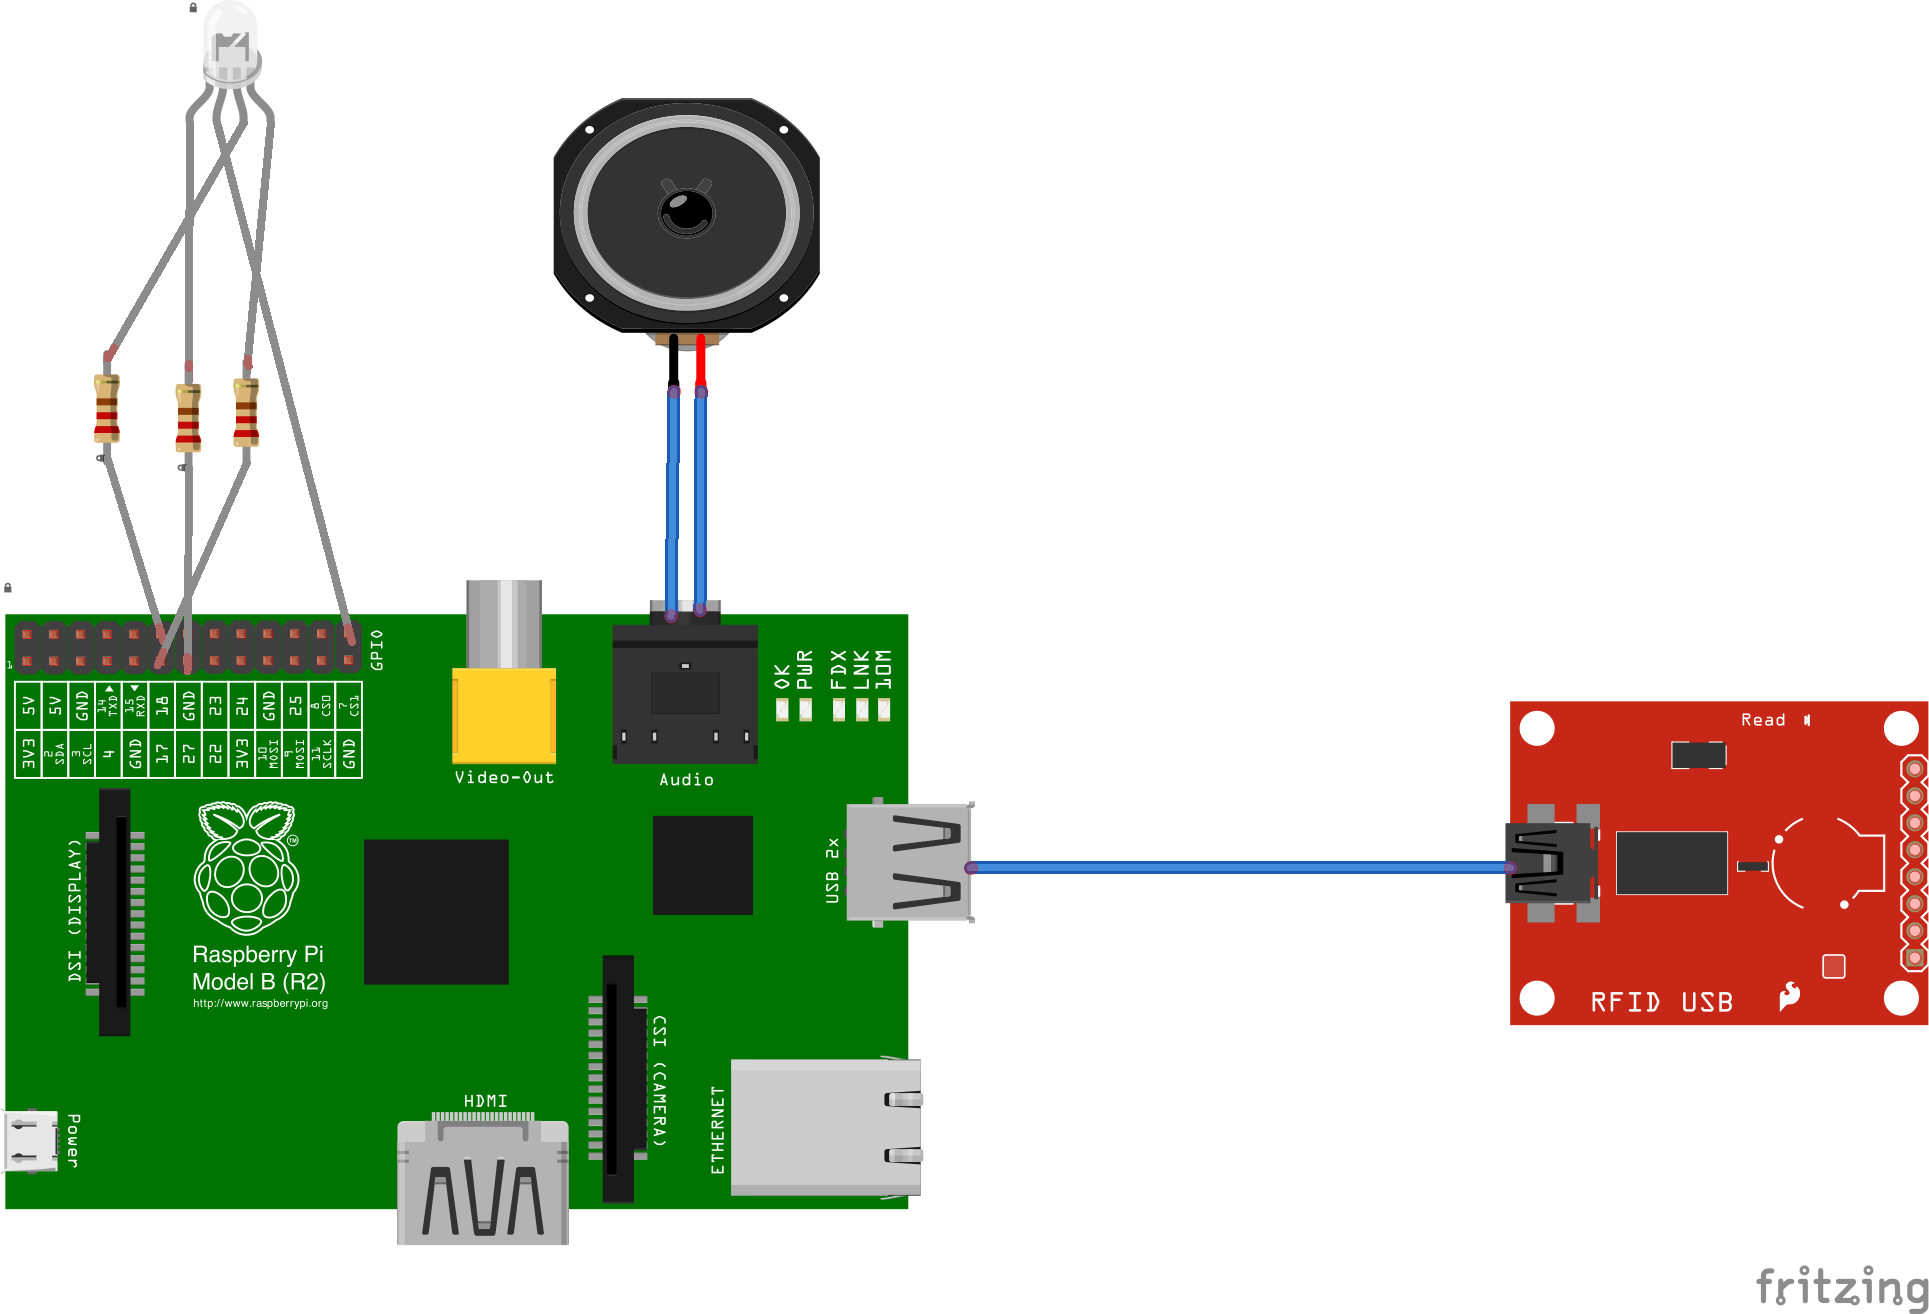
\includegraphics[width=0.3\paperwidth]{Pictures/pi-fritzing-model.png}}
		\caption{Digital schematic of the components}
		\label{fig:pi-fritzing}
	\end{minipage}
\end{figure}
 
  
\subsection{Additional Components}
\label{sec:additionalcomponents}
In addition to the \rpi{} we needed some components that children are able to interact through. These components and their functionality are summarized in this section. 


\textbf{RFID Reader}

In order to interact with \ab{}, children can register RFID-tags against \ab{}'s stomach. The RFID-reader we used was a Sparkfun ID-12LA\fnurl{Sparkfun ID-12LA documentation}{http://tiny.cc/sparkfundoc}. Our requirements when choosing a reader was that it should be able to connect through an USB-port, and be able to communicate with UNIX-systems.
         
\textbf{USB speakers}

In order to play sounds we decided to integrate speakers inside AsthmaBuddy. Since we did not want to pull too many wires out of the bear, we decided to use USB-powered speakers.    


\textbf{LED lights}

We used LED lights connected to a breadboard in order to play around with the first prototype. The LED lights emits light in different colors to correspond to what action(s) is expected from the user during a treatment (see more in Section \ref{sec:proto1}). 

In order to display the correct colors to the child, according to the color of the medicine, we tried to use PWM\fnurl{Pulse-width Modulation}{http://en.wikipedia.org/wiki/Pulse-width\_modulation}. However, these experiments resulted in a significant weaker light. Thus, we used a simple combination of blue and red in order to display purple, and a combination of red and green to display orange.  

 
Figure \ref{fig:pi-fritzing} shows a digital overview of \buddy{}. The green figure to the left is our \rpi{}. While it is also connected to a power supply and an internet cable, we chose not to include these in our figure. The red figure to the right is the RFID reader. It is connected to the \rpi{} through a USB cable. The black figure on top is the speaker, connected to the \rpi{} through the audio port. 
The grey lines and the lamp represents our LED light. It is connected to three of the GPIO (General Purpose I/O) ports on the \rpi{}, through a resistor. The last leg of the LED light is connected to ground on the \rpi{}, without a resistor.

A complete guide for wiring the components and running the application is included in Appendix \ref{app:asthmabuddy_manual}.

\subsection{Components Considered for Use}
\label{sec:componentsconsidered}
In addition to the components mentioned in the last section, we considered using buttons, touch sensors and a microphone. Even though we did not use these components, we simulated them during user tests using the Wizard-of-Oz technique. 

\textbf{Buttons}

One or more buttons could have been used on \ab{}. Buttons could have been used to manage boolean values, for instance if the progression of an instruction needed a yes/no answer. We did not include buttons, as it could disturb the impression of \ab{} as a regular teddy bear, i.e. it would seem more mechanical. 

\textbf{Touch sensors}

A touch sensor could serve the same purpose as a single button. We did not include this component, as it would require a set of low level programming skills. 

\textbf{Microphone}

A microphone could be used for speech recognition purposes. However, the \rpi{} does not have the processing power required to do speech recognition. Additionally, it would require writing code that is able to distinguish between noises\footnote{We were not able to find any open source libraries that are able to do speech recognition for the Norwegian language}. We thought it could have been a cool feature that would help establishing a relationship between the user and \ab{}, but we found it infeasible to implement given our limited time and resources.    

\subsection{Frameworks and Libraries Used in \ab{}} 

\textbf{Pi4j}

We wanted to write the code on our \rpi{} in Java, as it was our most familiar programming language. It is, however, cumbersome to use \rpi{}'s GPIO-ports and serial communications with native Java. Pi4j\fnurl{Pi4j}{http://pi4j.com} solved this problem, by making the necessary hardware abstractions.

\textbf{Gson}

Refer to Chapter \ref{sec:techandframeinapp} for a description of Gson.    

\textbf{JLayer}

JLayer\fnurl{Javazoom JLayer}{http://www.javazoom.net/index.shtml} is an open source MP3 decoding library. We used it to play back audio tracks on the \rpi{}. It is an old project, and might be out dated, but it served its purpose for our research.  
 

\section{Design Rationale}
\label{sec:designrationale}
\subsection{Why a Teddy Bear?}
When designing \buddy{} we chose a teddy bear as an avatar for our system. There are several reasons as to why we think a teddy bear is an appropriate avatar: Teddy bears are well known toys, and have been loved by children for a long time. They are considered gender-neutral\cite{stagnitti1997determining}\cite{cherney2006gender} and in our subjective opinion it is a toy that could be discretely placed in a child's room. With the appearance of a teddy bear, \buddy{} can easily be placed among other toys and not stand out. It was also important for us to choose a teddy bear of some size. A too thin a bear could lead to problems when fitting the system inside the bear, and could be met with scepticism by the children. \buddy{} will have similarities to Tamagotchi\cite{tamagotchi} and Furby\cite{furby}, but \buddy{}'s purpose is to motivate, instruct and teach children about asthma, not be a toy purely for playing with. 

While designing our system we also wanted to make sure that our system did not have robot-like features or robotic similarities. While children tend to find technology very interesting, we wanted to make \buddy{} seem as natural as possible, making a stuffed toy animal, rather than a technological toy. We believe that these design choices served our purpose of making children more aware of their asthma, while not being a constant reminder and a stress element. 

Norwegian fire fighters have used a teddy bear in order to calm down children who find themselves in dramatic situations\fnurl{NRK: Firefighters use teddy bears to calm down children}{http://www.nrk.no/trondelag/bamser-i-utrykningsbilene-1.11548966}. The fire fighters state that the children respond positively to the teddy bear. 
While we were not able to find scientific research done on the use of teddy bears in dramatic situations, we found this news article interesting and worth mentioning in our research. 

A teddy bear has also been used as an avatar for giving instructions on how to apply a treatment correctly. Glaxo Smith Kline, a leading company within consumer health care, uses a teddy bear in their instruction manual for the use of asthma medicine and the breathing chamber\cite{glaxosmithkline}. 

Below are two pictures of how \ab{} looks in its final form. 

\begin{figure}[H] 
	\begin{minipage}[t]{0.4\linewidth}
	\centering
		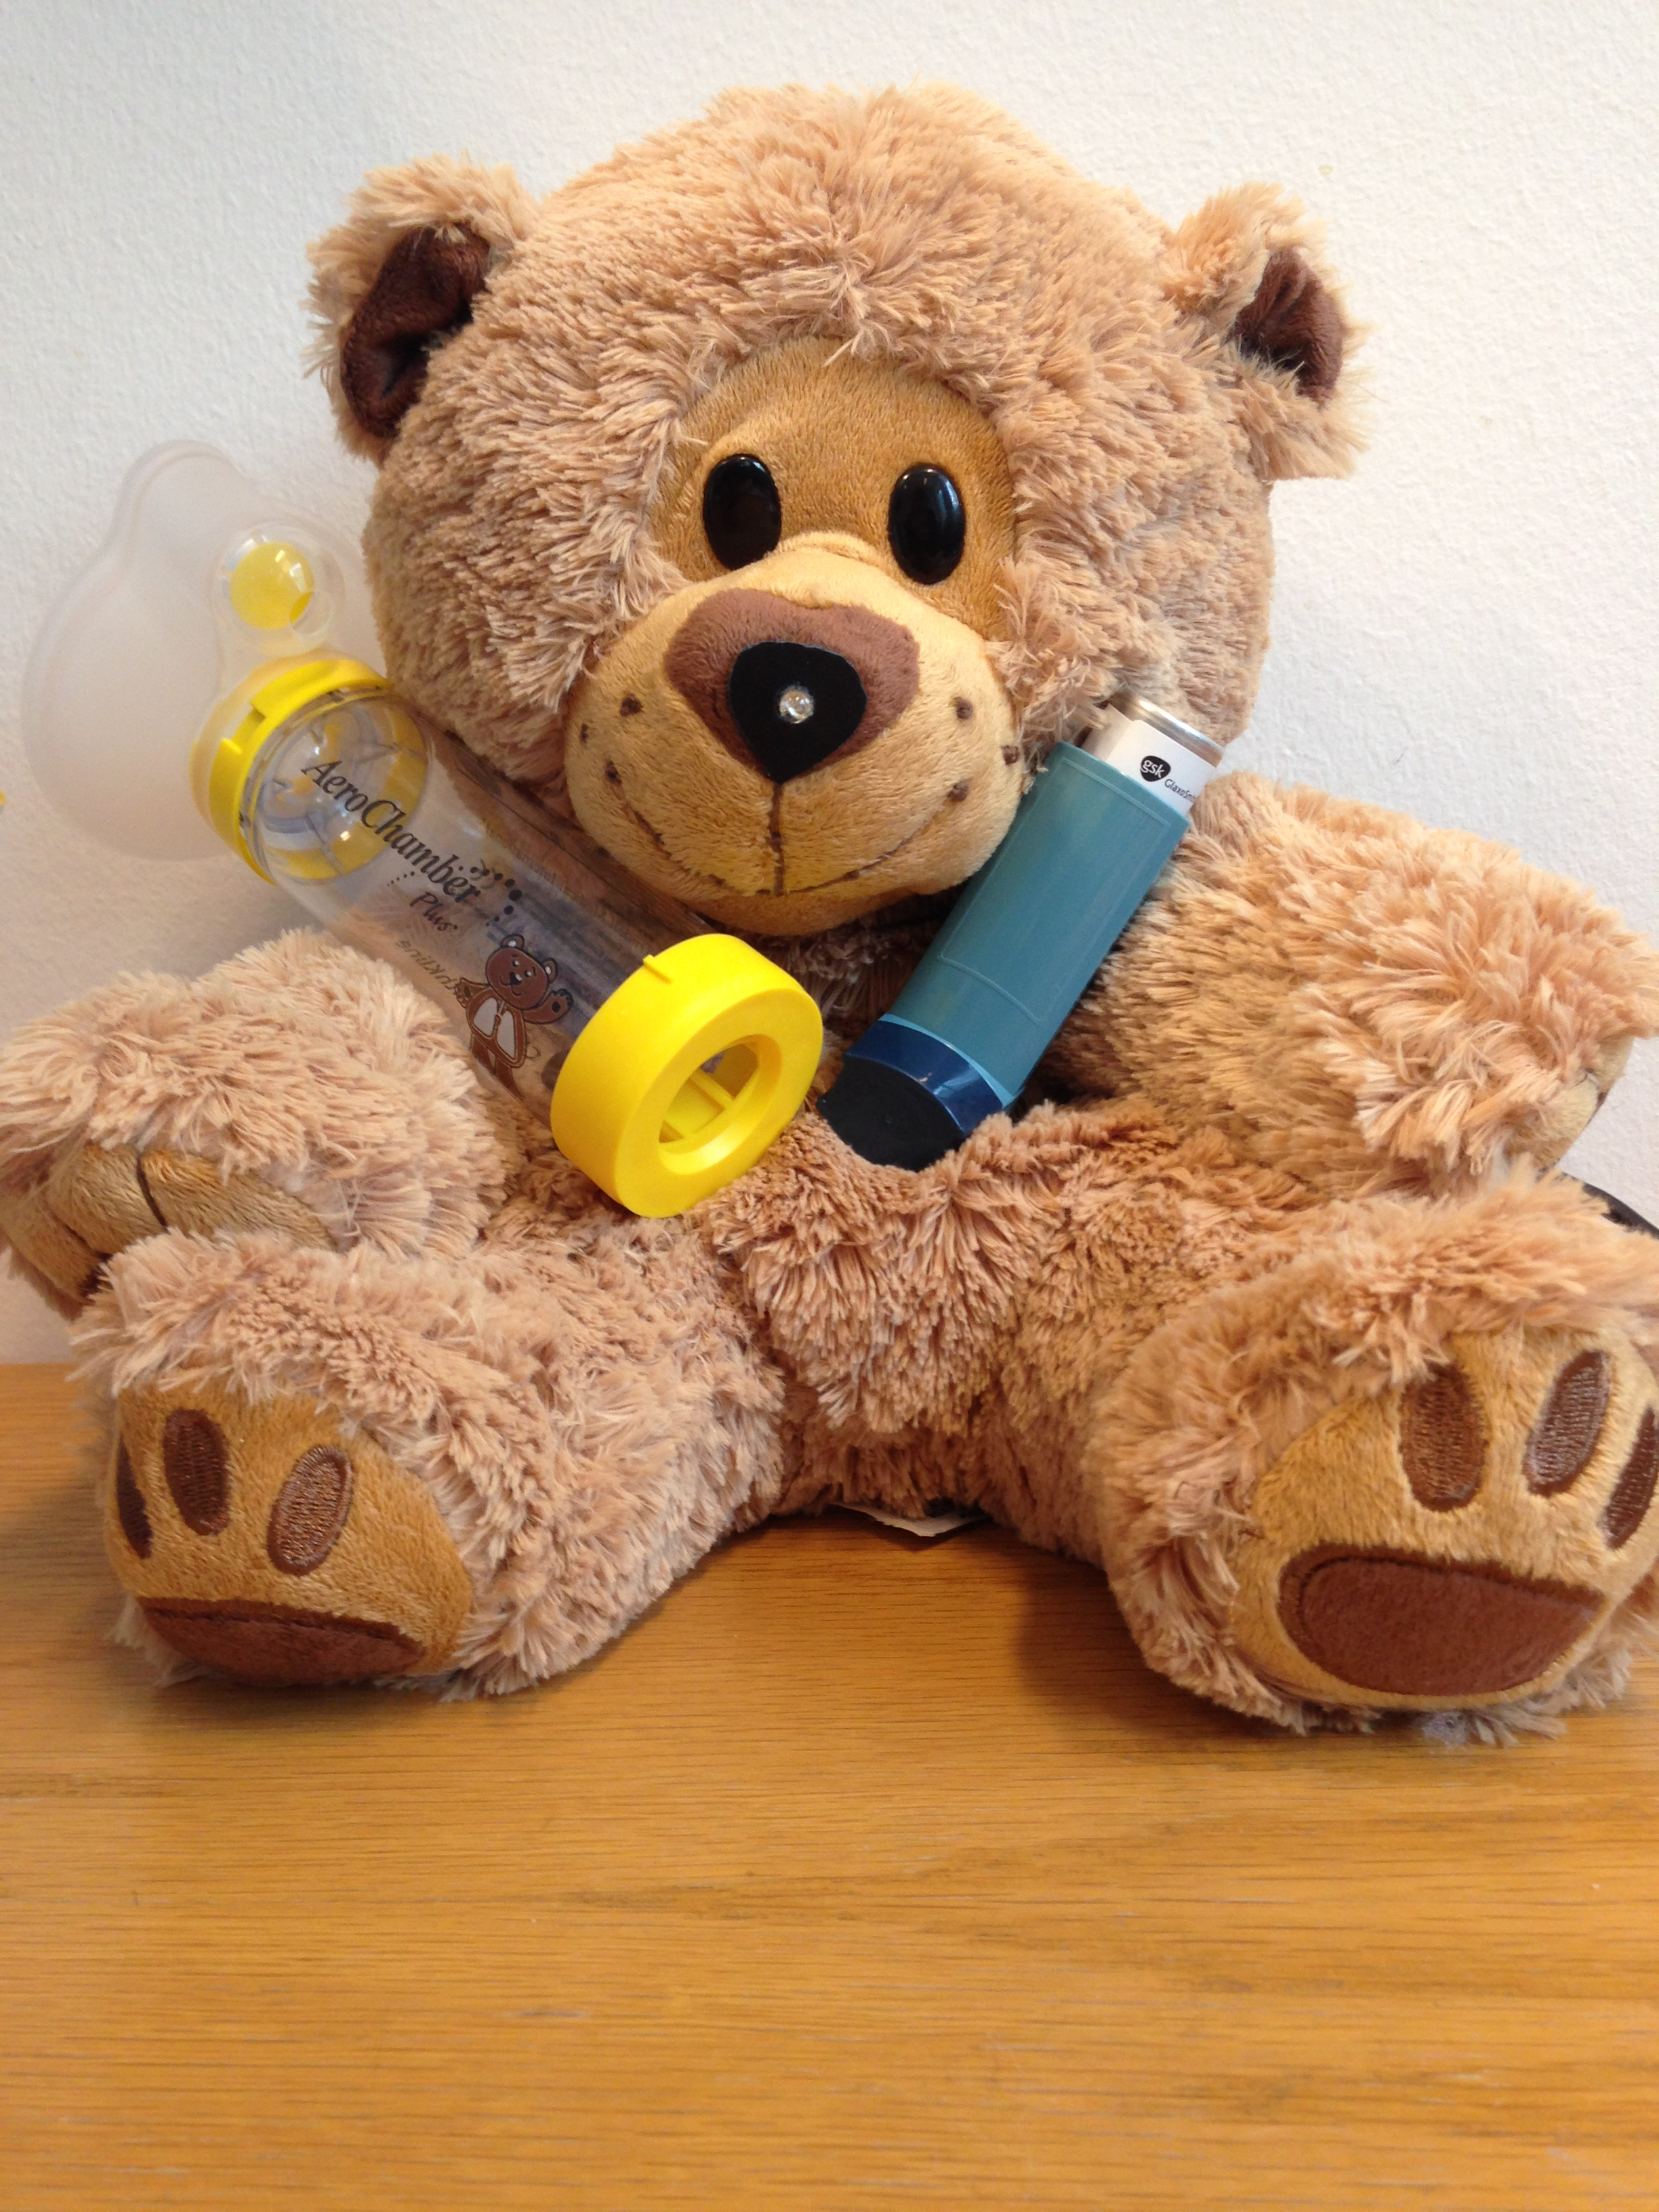
\includegraphics[width=0.3\paperwidth]{Pictures/abandinhaler.jpg}
	\caption[AsthmaBuddy holding a breathing chamber and an inhaler]{AsthmaBuddy holding a breathing chamber and an inhaler}
	\label{fig:asthmabuddyandinhaler}
	\end{minipage}
	\hspace{2.0cm}
	\begin{minipage}[t]{0.4\linewidth}
		\centering
			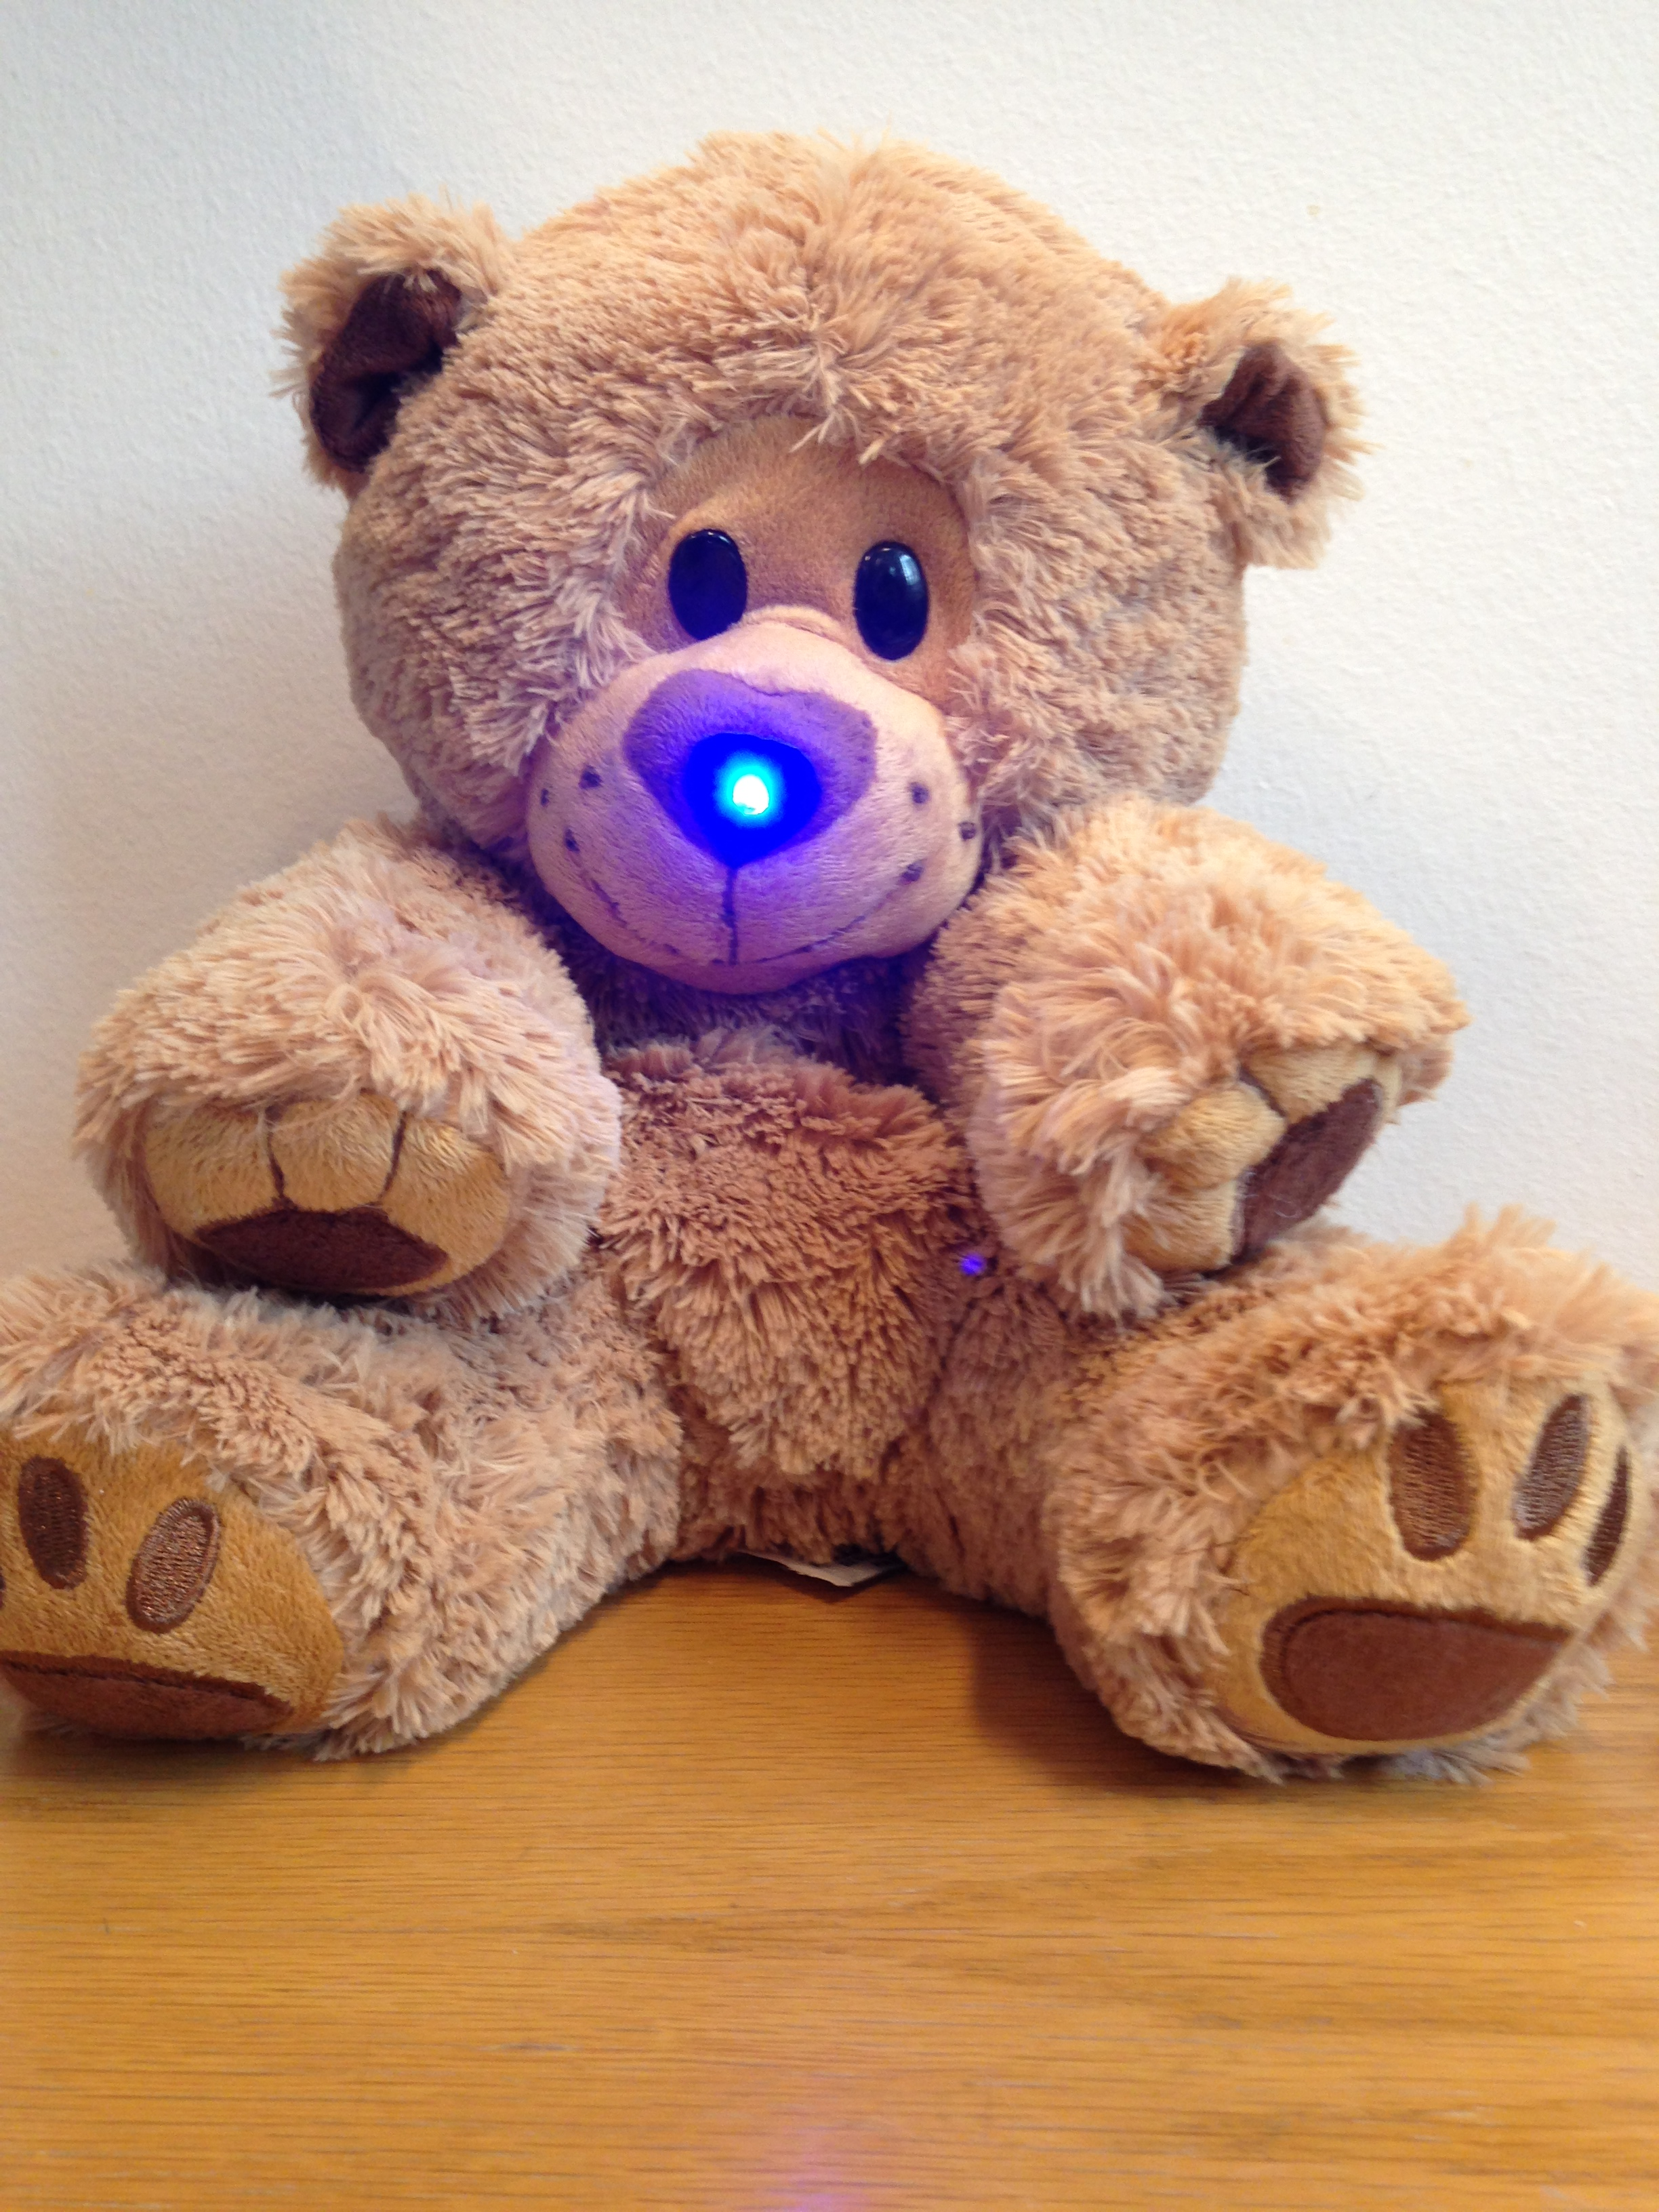
\includegraphics[width=0.3\paperwidth]{Pictures/abbluelight.jpg}
		\caption{AsthmaBuddy with his nose light turned on}
		\label{fig:asthmabuddyandlightnose}
	\end{minipage}
\end{figure}


\subsection{Interaction Design}
\label{sec:interactiondesign}
When we started developing the interaction design of \buddy{}, we had a brainstorming session with the intention of coming up with reasonable interaction patterns.        
By ``reasonable'', we imply that the underlying functionality should be relatively cheap to implement. The interactions should also be fun for the children to perform, in addition to being efficient. 

\begin{singlespacing}
\begin{table}[H]
	\centering
	\begin{tabular}{| p{3.0cm} | p{5.0cm} | p{5.0cm} |}
		\hline
		\textbf{Interaction Process} & \textbf{Rationale} & \textbf{Possible implementation} \\
		\hline
		Give \buddy{} a ``High five'' & Demonstrates to children that \buddy{} is friendly. It is intended that a child should hold \buddy{}'s arm up, and high five \buddy{} with his hand. & A gyroscope and a preassure sensor combined could verify that a high five has been received. \\
		\hline
		Hold \buddy{}'s hand & Demonstrates to children that \buddy{} is friendly. & Preassure sensor within the hand of \buddy{} could solve this. \\
		\hline
		Hold smartphone close to AsthmaBuddy's belly & Could demonstrate the ``smartness'' of \buddy{}, i.e. it can communicate with other devices. & Could be solved by Bluetooth. \\
		\hline 
		Press \buddy{}'s nose & Demonstrates to children that \buddy{} is friendly. & Preassure sensor within the nose of \buddy{} could solve this. \\
		\hline
		Press \buddy{}'s belly & Demonstrates to children that \buddy{} is friendly. & Preassure sensor within the belly of \buddy{} could solve this. \\
		\hline
		Hold medicine close to \buddy{}'s mouth & Demonstrates that \buddy{} also needs his medicine. & An RFID-tag attached to the medicine, and an RFID-reader inside the nose of \buddy{} could be used here to control the flow. \\ 
		\hline
		Hold RFID-tag close to \buddy{}'s mouth & Is a relatively easy way to proceed with the process. & A loose RFID-tag could be used together with an integrated RFID-reader, in order to proceed. \\ 
		\hline
		Hold RFID-tag close to \buddy{}'s belly & Is a relatively easy way to proceed with the process. & A loose RFID-tag could be used together with an integrated RFID-reader, in order to proceed. \\
		\hline
		Clap your hands & Should be a fun way of interacting with systems, considering the age of our target group. & Sound recognition could be used here. \\ 
		\hline
		Combination of the interactions above & Makes the process more fun through variation. & N/A \\
		\hline
	\end{tabular}
	\label{tab:interaction-rationale}
	\caption{Rationale behind \buddy{}'s interaction design}
\end{table}
\end{singlespacing}

\subsection{Answering to Champoux's Development Framework}
\label{sec:answeringchampoux}
In Chapter \ref{sec:champoux} we described the development framework presented by Champoux \etal{} When developing \buddy{}, we tried to answer the proposed questions that we considered relevant. 

\textbf{BO1: What should the user experience?}
The user should experience an interactive guide for correct application of asthma treatment. \buddy{} should give correct information in an understandable manner. 


\textbf{BO2: What are the human tasks?}
\begin{itemize}
  \item Fetch an adult
  \item Fetch inhaler and breathing chamber
  \item Shake medicine
  \item Attach the inhaler to the breathing chamber
  \item Put the breathing chamber on your face, covering nose and mouth
\end{itemize}

\textbf{BO3: What should the artefact represent and control?}
\buddy{} represents a caregiver, who supervises the child during the treatment. The artefact controls that the child takes the medicine at the correct time, and in a correct manner.   

\textbf{BO4: What are the conventions?}
Children must have their inhaler and breathing chamber stored within a short distance of \buddy{}. The RFID-tags are assumed to be attached to the inhalers.    

\textbf{OC5a: What is the nature of the interaction for each sub-task (Continuous vs Discrete vs Assembly)?}
The sub-tasks performed when taking a medicine are the following:
\begin{enumerate}
  \itemsep0em
  \item Fetch an adult
  \item Fetch inhaler
  \item Fetch breathing chamber
  \item Prepare medicine
  	\begin{enumerate}
  	  \itemsep0em
  	  \item Shake the inhaler
  	  \item Attach inhaler to the breathing chamber
  	 \end{enumerate}
  \item Inhale dosage
  	\begin{enumerate}
  	  \itemsep0em
  	  \item Hold medicine towards mouth
  	  \item Press the inhaler
  	  \item Breathe heavily for 10 seconds
  	 \end{enumerate}
  \item Optional, depending on the medicine: Rinse mouth
\end{enumerate}

Step 4 is an assembly task, 5(c) is a continuous task for a short period of time, while the remaining tasks are all discrete.  

\textbf{OC6: Does the sub-task need any relational interaction?}
None of the described sub-tasks needs relational interaction. However, registering the RFID tag can be seen as a relational interaction, as the proximity of the RFID tag and the reader is essential.  
 
\subsection{Dealing with Bellotti's Challenges}
\label{sec:dealingwithbellotti}

Chapter \ref{sec:challenges-with-TUI} introduced some of the challenges that are encountered when designing tangible interfaces. In the following we will discuss how we handled the challenges encountered, by answering those of Bellotti's questions which we found relevant. 

\textbf{Address: How do I address one of many possible devices?}

One of the challenges mentioned here is ``How to not address the system''. This is an interesting challenge when the system is intended for children, as they are likely to pick things up and carry them around. If a child picks up \ab{}, it could be interpreted as an interaction. We solved this potential problem by only starting treatments in one of two ways, either because it is triggered by an alarm or because an RFID-tag attached to an inhaler is read by \ab{}. The RFID-reader is only capable of reading the tag from a distance of 3 - 5 cm. Thus, as long as no alarm is triggered, and no inhaler with attached RFID-tag is not withing the reach of the RFID-reader, the system should not respond.  


\textbf{Attention: How do I know the system is ready and attending to my actions?}

As mentioned previously, \buddy{} has a LED-light on it's nose. When the light is green, the user can expect that the system is running in idle mode. 

\textbf{Action: How do I effect a meaningful action, control its extent and possibly specify a target or targets for my action?}

The part that regards specifying a target or several targets is considered irrelevant. The interesting part is how the user can effect a meaningful action and control its extent. This will be taken care of by interactions between the user and \buddy{}. \buddy{} will never run several instructions at once. It will always give short and clear instructions, and wait for feedback from the user in order to proceed. 

\textbf{Alignment: How do I know the system is doing the right thing?}

By listening to \buddy{} speak, the user should be aware of what is happening. There is not a lot of room for human error in this connection. By following the normal sequence of operation, the worst thing that may happen is a system crash. This will be handled by shutting down the lights, and \buddy{} will not be running.  

\textbf{Accident: How do I avoid mistakes?}

A part of the challenge is to recover from mistakes that have occured. For instance, if the user proceeds further than what was actually intended, and missed out on an instruction they needed, \buddy{} should have a way to revert to the missed instruction. \ab{} has functionality to replay instructions, but it needs to be told to do so by keyboard input from the ``Wizard-of-Oz''. During user tests, children were told to say ``Repeat'' loud and clear, in order to replay an instruction. Moving beyond the ``Wizard-of-Oz'', this could be handled by a separate form of interaction, e.g. shaking \ab{}'s head, in order to make him repeat the instruction.      
\section{Use of Gamification in \ab{}}
\label{sec:useofgamificationinab}
\ab{} works together with \app{} to create our gamification system. While \app{} handles the support for creating and purchasing rewards, \ab{} is able to reward children with stars and keep track of how many stars the child has collected. 
When finishing a treatment, the child is told how many stars he/she collected for finishing the specific treatment. \ab{} states ``Well done. As a reward, I'll put N stars in your treasure chest'' where N is replaced by  1, 3 or 5, based on the health state of the child. Afterwards, the child is told ``You have now collected M stars'' where M is replaced by the total amount of stars the child has collected. 

\ab{} also supports telling the user how many stars have been collected without having to go through a treatment first.


\section{System Overview}
\label{sec:systemoverview}

\subsection{Use Cases}
Figure \ref{fig:pi-use-cases} shows a general overview of the use cases we have included in our prototype. A medication process can be started set off two ways:
A parent can register an alarm by using AsthmAPP. This alarm is then set of by the \code{AsthmaBuddy} instance running\footnote{The reader should take notice that the tangible user interface \ab{} differs from the program running on the \rpi{}, which is called \code{AsthmaBuddy}(note the change of font)}, giving the child a notification that it is time to take the relevant medicine.

The alternative to a registered alarm is if a child needs to take the medicine by need. In such case, the child or parent simply registers the RFID-tag before the child is guided through a quicker process (see Manuscript \ref{chp:anuscript}).  

\begin{figure}[H] 
	\centering
		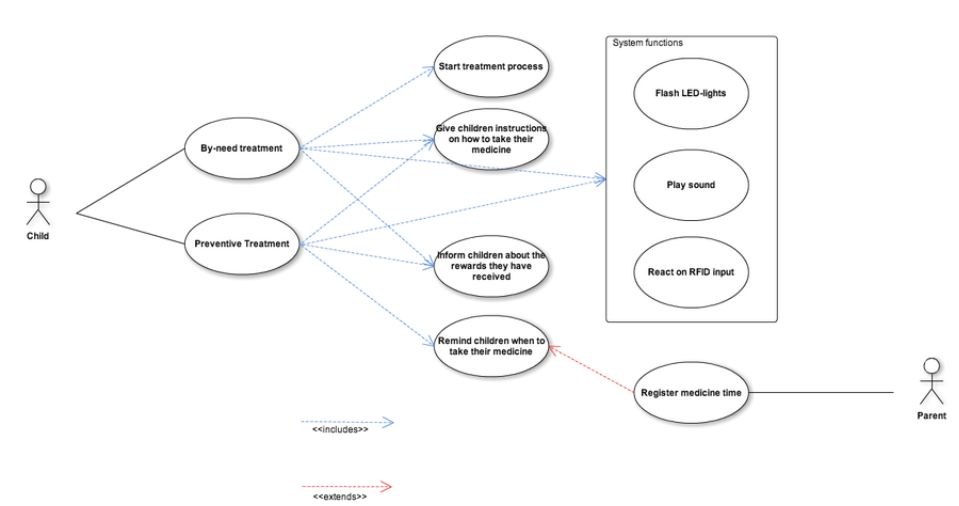
\includegraphics[width=0.8\paperwidth]{Pictures/usecases.png}
	\caption{AsthmaBuddy Use Cases}
	\label{fig:pi-use-cases}
\end{figure}

\subsection{Textual Use Cases}
\label{sec:textualusecasebyneed}

%--------- TEXTUAL USE CASE ----------
%--------- BY NEED TREATMENT ---------
\begin{table}[H]
\centering
\begin{tabular}{|p{4.0cm} | p{9.0cm} |}
\hline
\textbf{Title} & By need treatment \\
\hline
\textbf{Preconditions} & - \\
\hline 
\textbf{Scenario} & 
	\begin{enumerate}
	  \itemsep0em
	  \item User triggers treatment by holding a specific RFID-tag close to AsthmaBuddy.
	  \item System flashes LED-lights to notify user that the system is ready for use.
	  \item System plays sound to instruct the user to shake the medicine.
	  \item System plays sound to instruct user to mount the medicine on the mask and place the mask on his/her face.
	  \item User starts a treatment by interacting with AsthmaBuddy (by pressing it's hand or similar interaction).
	  \item System plays sound to count during treatment (1-2-3-4-5-6-7-8-9-10), while flashing lights for each count.
	  \item System plays sound to tell user he/she has done a good job.
	  \item System calculates reward based on health state.
	  \item System plays sound to award user with the calculated number of stars.
	  \item System plays sound to tell the user how many stars he/she has collected totally.
	\end{enumerate}
\\
\hline
	\textbf{Extensions} & 
		x.a User aborts treatment by not continuing the sequence.
\\
\hline
\end{tabular}
\caption{Textual use case: By need treatment}
\label{tab:textual-use-case}
\end{table}


%--------- PREVENTIVE TREATMENT -------

\begin{table}[H]
\centering
\begin{tabular}{|p{4.0cm} | p{9.0cm} |}
\hline
\textbf{Title} & Planned treatment \\
\hline
\textbf{Preconditions} & The current time corresponds with the time for a planned treatment. \\
\hline 
\textbf{Scenario} & 
	\begin{enumerate}
	  \itemsep0em
	  \item The system recognizes the time for a planned treatment.
	  \item The system starts blinking with LED-lights and playing sound to notify user.
	  \item Child interacts with AsthmaBuddy, to notify that he/she is ready for the treatment.
	  \item Start instructions by playing sound, telling the user to find a grown-up that can keep watch.
	  \item System waits for interaction to make sure the user is ready.
	  \item System tells the user to mount the medicine on the mask and put the medicine towards AsthmaBuddy's face.
	  \item System plays sound to simulate breathing.
	  \item System plays sound to tell the user how easy it was to take medicines and that it is the user's turn.
	  \item System plays sound to instruct user, telling the user to shake the medicine.
	  \item System waits for interaction to make sure the user is ready.
	  \item System plays sound to instruct user to put the mask on his/her face.
	  \item System plays sound counting to 10. 
	  \item System plays sound to tell the user he/she has done a good job.
	  \item System calculates reward based on health state.
	  \item System plays sound to award user with the calculated number of stars.
	  \item System makes a HTTPGet call to the server to find the total number of stars collected.
	  \item System plays sound to inform the user about how many stars the user has collected totally.
	\end{enumerate}
\\
\hline
	\textbf{Extensions} & 
		x.a Child does not interact with AsthmaBuddy when prompted
\\
\hline
\end{tabular}
\caption{Textual use case: By need treatment}
\label{tab:textual-use-case}
\end{table} 


\subsection{State Diagram}
\label{sec:statediagram}

In order to start the AsthmaBuddy application, we used SSH in order to gain access to the computer. We then retrieved the latest version of the source code from Git\fnurl{Git is the Source Code Management system we used}{http://git-scm.com/}, compiled it, and started running it (this process is described in Appendix \ref{app:asthmabuddy_manual}). Once AsthmaBuddy is running, it follows the state diagram depicted in Figure \ref{fig:asthmabuddy_statediagram}.  
  

\begin{figure}[H] 
	\centering
		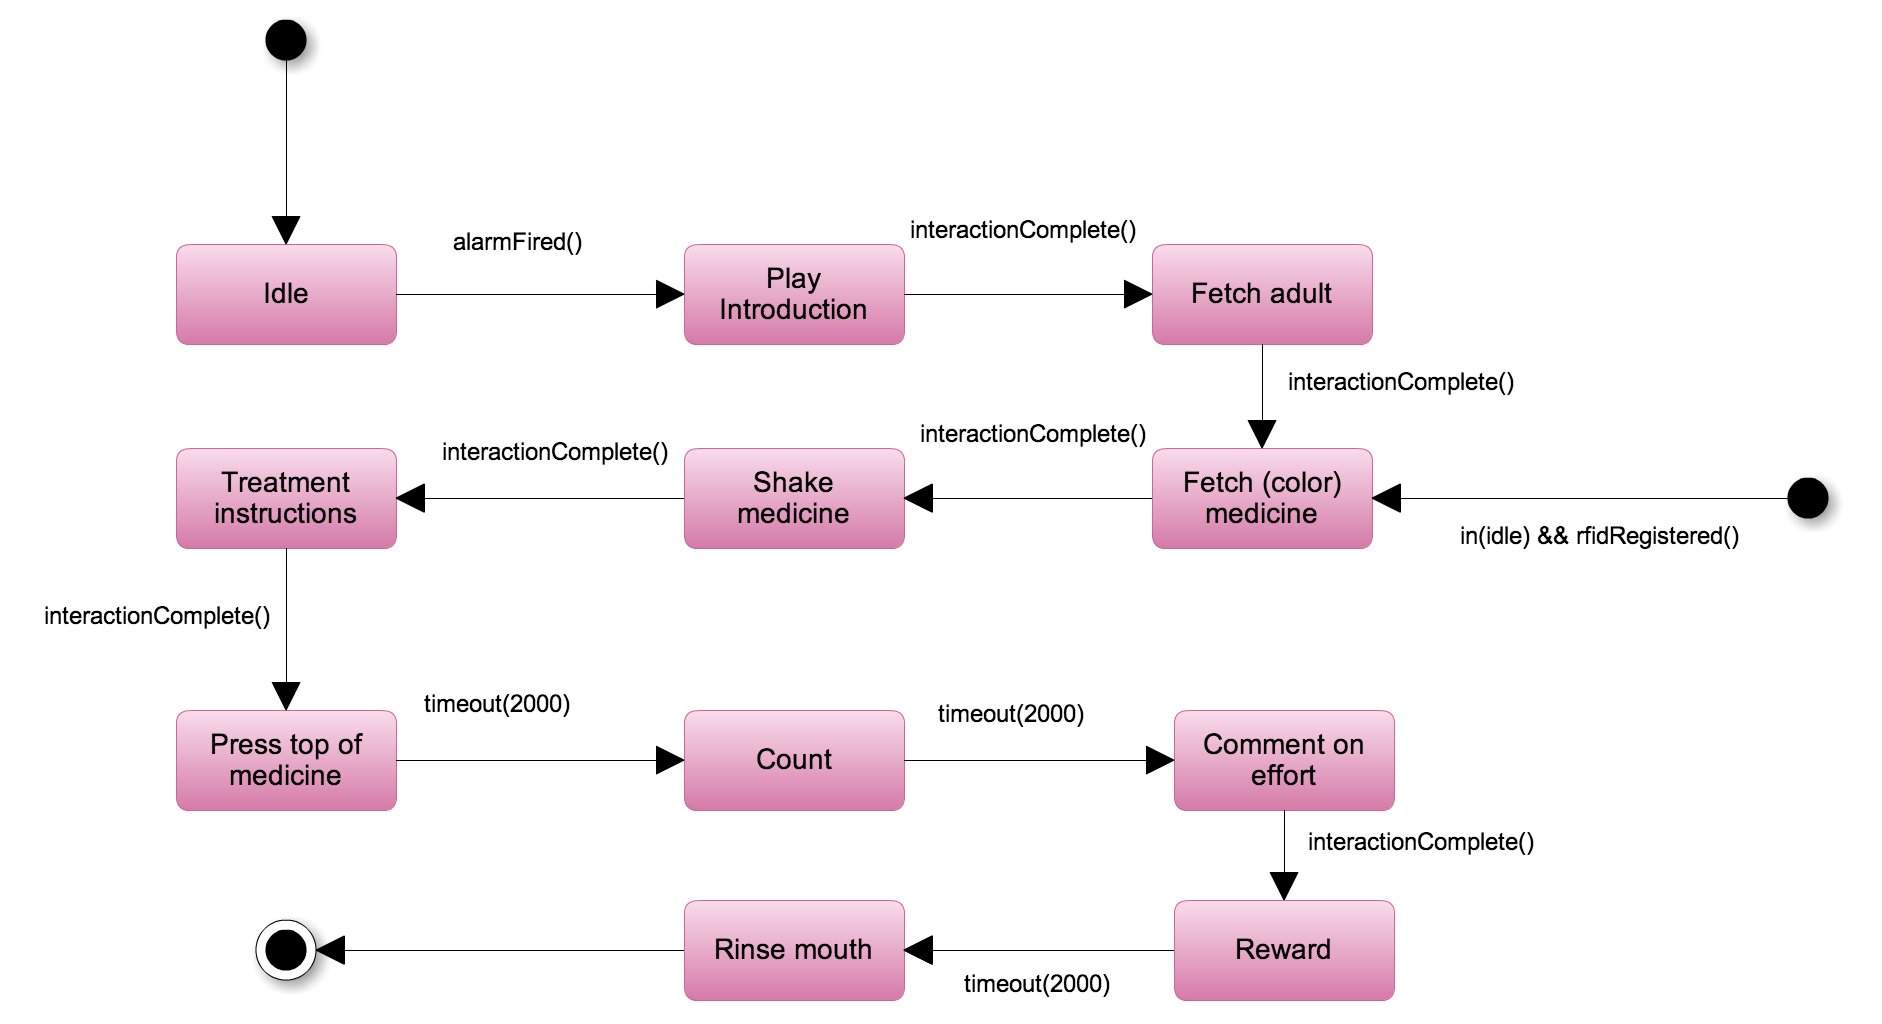
\includegraphics[width=0.7\paperwidth]{Pictures/statediagram.png}
	\caption{AsthmaBuddy State Diagram.}
	\label{fig:asthmabuddy_statediagram}
\end{figure}

\subsection{Sequence Diagram}
Figures \ref{fig:ab-sd-byneed} - \ref{fig:ab-sd-completing-treatment} shows sequence diagrams of how the system works internally. Some abstractions have been made, in order to reduce the cluster of arrows. 

\begin{sidewaysfigure}[htbp]
	\centering
		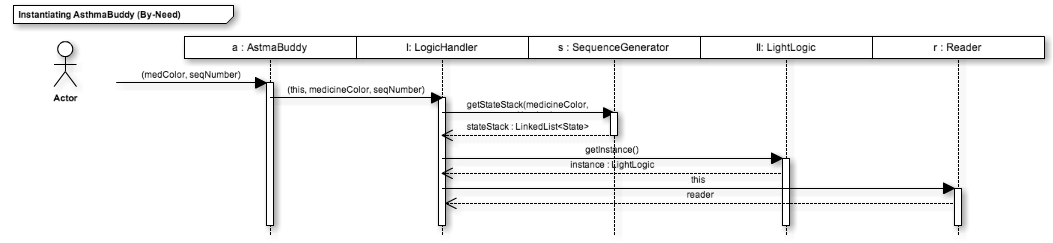
\includegraphics[scale=0.6]{Pictures/sd/sd-byneed.png}
	\caption{By Need Treatment - Sequence Diagram}
	\label{fig:ab-sd-byneed}
\end{sidewaysfigure}

\begin{sidewaysfigure}[htbp]
	\centering
		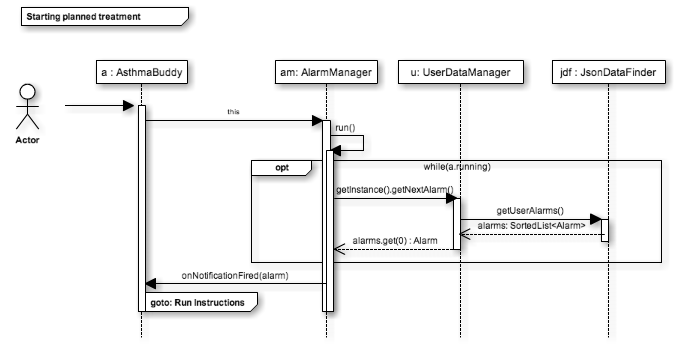
\includegraphics[scale=0.6]{Pictures/sd/sd-planned-treatment.png}
	\caption{Planned Treatment - Sequence Diagram}
	\label{fig:ab-sd-planned-treatment}
\end{sidewaysfigure}

\begin{sidewaysfigure}[htbp]
	\centering
		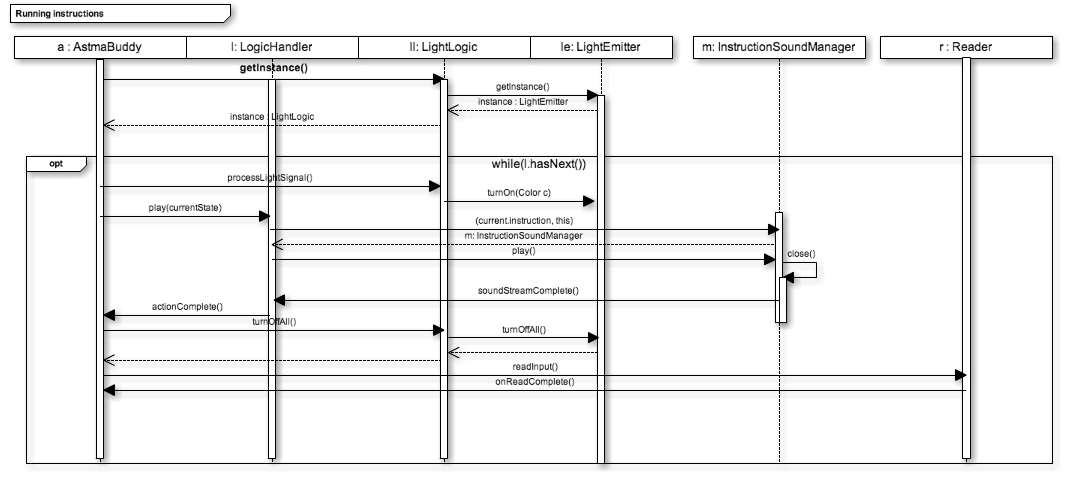
\includegraphics[scale=0.6]{Pictures/sd/sd-instructions.png}
	\caption{Playing Instructions - Sequence Diagram}
	\label{fig:ab-sd-instructions}
\end{sidewaysfigure}

\begin{sidewaysfigure}[htbp]
	\centering
		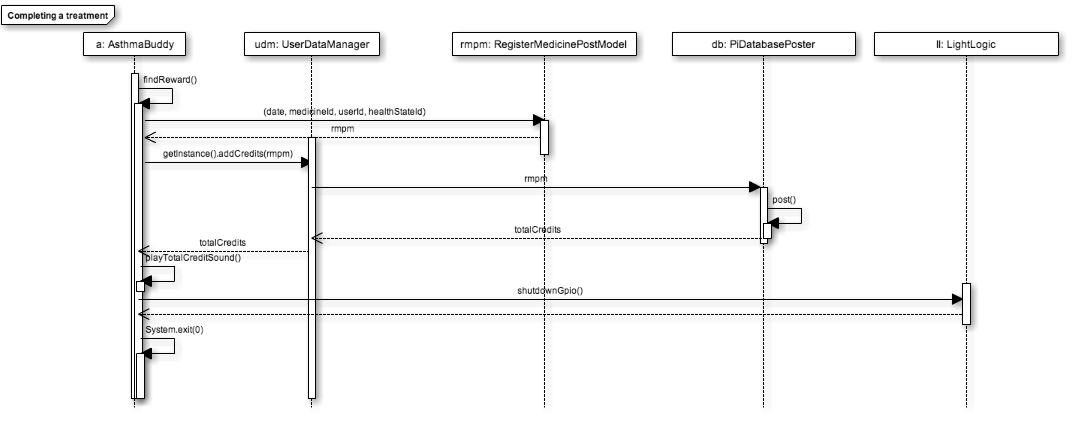
\includegraphics[scale=0.6]{Pictures/sd/sd-complete-treatment.png}
	\caption{Finishing a treatment - Sequence Diagram}
	\label{fig:ab-sd-completing-treatment}
\end{sidewaysfigure}


\begin{sidewaysfigure}[htbp]
	\centering
		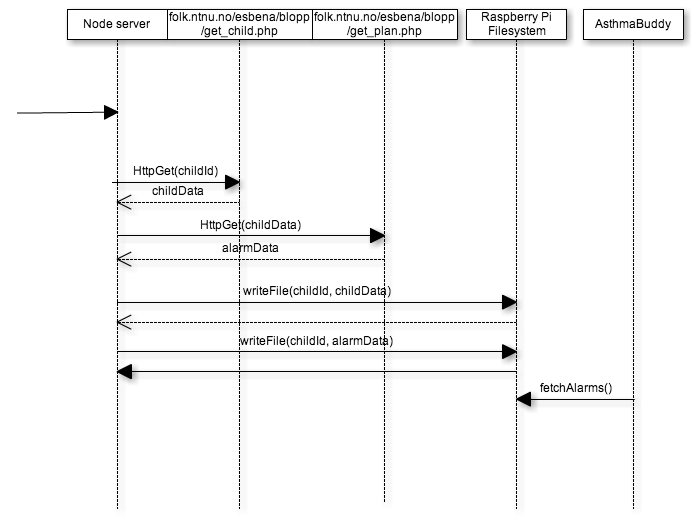
\includegraphics[scale=0.6]{Pictures/sd/sd-synchronizingv2.png}
	\caption{Synchronizing alarms - Sequence Diagram}
	\label{fig:ab-sd-synchronizing}
\end{sidewaysfigure}

\textbf{By Need Treatment}

We were not able to find a reasonable easy way to let the \buddy{} automatically be aware of the medicine that was to be taken at the start of a treatment. As a result, we used ssh into the \rpi{}, and provided the color of the medicine and the sequence number for the interaction that was to be tested.

After inserting these parameters, the \code{LogicHandler} retrieves a \code{LinkedList} of \code{Interaction}-objects that is to be played. After this sequence is ended, the system jumps to Figure \ref{fig:ab-sd-instructions}.
 
\textbf{Planned Treatment}

If an \code{AsthmaBuddy} instance is started without any parameters, it starts looking through alarm files (see Section \ref{sec:node-server}) every 60 seconds. If no alarm is returned from \code{UserDataManager}, it waits. Once an alarm is found, \code{AsthmaBuddy} is notified through \code{onNotificationFired}, which starts the treatment process. 
 
\textbf{Playing Instructions}

Playing instructions is mainly a loop of playing a sound, and turning on and off the LED-lights through the \code{LightEmitter} instance. 

\textbf{Finishing a Treatment}

When a treatment is finished, i.e. we are out of the \code{while} loop in Figure \ref{fig:ab-sd-instructions}, we register the treatment in the database. This ensures that the child is able to see the rewards in AsthmAPP. 


\subsection{Node Server}
\label{sec:node-server}
In addition to the Java application running on the \rpi{}, we developed a Node.js server\fnurl{Node.js}{http://nodejs.org/}. This backend system was developed in order to easily visualize the rewards given to a child after a treatment using \buddy{}. The initial problem is that AsthmAPP stores data to a MySQL database, with \code{childId} as the primary key for most tables. Initially, \buddy{} has no way of knowing which \code{childId} to add rewards to, or for which user alarms should be triggered. The current solution to our problem was to develop a Node.js server on AsthmaBuddy, which run as a background process. Whenever we want to switch users, AsthmAPP does an HTTP POST to this server, including the \code{childId} as a parameter. The server then retrives JSON-formatted data from our webservice, which includes the rewards a child has been given until now (for instance, by using a smartphone), and the alarms set for this user. 
When \buddy{} starts running, it checks for alarms to be set off every 60 seconds. When a child has finished a treatment, \code{AsthmaBuddy} updates the database, with the \code{childId} previously retrieved, and the number of stars a child collected during his/her treatment. With the data retrieved from the database, \buddy{} has the capability to tell the user how many stars a child has collected\footnote{Since this is a prototype, this functionality only works until a child has collected 20 stars. It became cumbersome to handle rewards totalling more than 20 stars}. This process is shown in Figure \ref{fig:ab-sd-synchronizing}.


 

\section{Prototype Version 1}
\label{sec:proto1}

Our first version of \ab{} was supposed to have capabilities to guide a child through a treatment. It was possible to interact with \ab{} through the interactions described in Table \ref{tab:interaction-rationale}. Version 1 did not have the ability to synchronize rewards with \app{}, nor informing the user about the total amount of stars collected. We tested the version on inexperienced users (results can be found in Chapter \ref{chp:interaction-methods}), in order to discover information flaws and difficulties when interacting with \ab{}. We assumed that if an adult was not able to perform a treatment correctly with \ab{}, then children would not be able to do it either.  

We did not have the resources available to implement all of the interaction methods listed. As such, we simulated the interactions through the Wizard-of-Oz technique\cite{wilson1988rapid}.

This version was also used for demonstration purposes during our interviews, which provided us useful feedback on functionality we could add to \ab{}.           
	
\section{Prototype Version 2}
\label{sec:abversion2}
The improved version of \ab{}, hereby referred to as \ab{} 2.0, had some changes done since version 1.0. After testing version 1.0 on inexperienced users, we removed some of the interaction methods. A summary of the interaction methods available in version 2.0 is provided in Chapter \ref{chp:interaction-methods}. \ab{} 2.0 is able to synchronize collected stars automatically between \app{} and \ab{}. This was done to automate some tasks that previously needed manual interaction, and to create a tighter coupling between the two prototypes.

\ab{} 2.0 also received some new features, such as a method for letting children more easily check the total amount of stars they have collected. By registering an RFID tag, \ab{} tells how many stars the child has. This was implemented to make \ab{} more of a stand-alone system, and to avoid the problem where parents may not want their child to use their smartphone to use \app{}. 
 
Additionally, some small changes were made to the use of the LED light on \ab{}'s nose. \ab{} 1.0 changed the color of its nose fairly often. This was intended to make the treatment process more interesting; however, it ended up being more confusing than helpful, and was therefore changed to mirror the breaths of the user, and the color of the medicine container. 

\section{Summary}
\label{sec:asthmabuddysummary}
We have developed a prototype for a tangible user interface called \ab{}, who can be used to guide a child through a treatment process. The software behind the prototype is built upon a \rpi{}, which was placed inside \ab{}. We designed a set of interaction methods that we considered appropriate for children. This set was narrowed down after a round of user tests on inexperienced users (see Chapter \ref{chp:interaction-methods}). It is currently capable of reading RFID tags, playing sounds and changing the light of its' nose. During the user tests, we simulated the usage of microphones with voice recognition, sensing touches to it's hand, sensing a smartphone's precence and distinguishing between a touch and a high five.       
